% LINKS IN STYLE FILE
\documentclass{ueacmpstyle}

% DIFFERENT PACKAGES THAT YOU MAY USE THROUGHOUT YOUR REPORT - LOOK AT OVERLEAF TUTORIALS ON DIFFERENT PACKAGES (i.e. tables)
\RequirePackage{natbib}
\usepackage{graphicx,caption}
\usepackage{subcaption}
\usepackage{appendix}
\usepackage[hyphens]{url}

\begin{document}
    % HEADER SECTION
	\title{Coursework of Foundations of Data Science (CMP-5046B)}    % COURSEWORK TITLE
	% \title{Human Computer Interaction -- Coursework 1} << Example Title
	\author{
		100241852\\     % Can just use student number but if you include name separate with double hyphen
		May 26 2021     % Module code here - use the code that is relevant to you
	}
	\maketitle
	
	\newpage

    \section{Introduction}\label{sec:introduction}
    
    This assignment aims to implement data science pipelines such as nearest neighbour and least squares approaches to evaluate regression models for real-world problem. This report will explain the results after performing data manipulation using Python libraries and make use of scatter plot and histogram to present the results. This report discusses statistical techniques such as simple regression and multiple regression that uses several independent (explanatory) variables to predict the dependent (target) variable. The results include standardised variables, correlations, performance metrics received from nearest neighbours and least squares in both simple and multiple regression and bootstrapping results.
    
    The regression problem for this assignment is based on QSAR model for predicting acute toxicity on fish (fathead minnow) \citep{ref_1}. The independent variables for this problem are the 6 molecular descriptors: MLOGP (molecular properties), CIC0 (information indices), GATS1i (2D autocorrelations), NdssC (atom-type counts), NdsCH ((atom-type counts), SM1\_Dz(Z) (2D matrix-based descriptors), which measures the concentration that causes death in fish during the test time-frame. The dependent variable is LC50 [-LOG(mol/L)] which is a response to the independent variable.
    
    \section{Description of data}\label{sec:description}
    
    The data contains result of 908 test sets retrieved from UCI Machine Learning site. The figure below displays the first 5 rows of the table. The first six columns are the independent variables x which will be used to predict the value of dependent variable y. The final column contains the actual result of y.
    
    \begin{figure}[!htb]
    	\centering
    	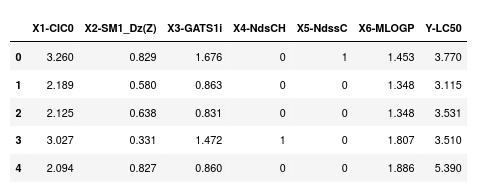
\includegraphics[width=0.5\textwidth]{qsar_data.png}
    	\label{fig1}	
    \end{figure}

	The graph below displays the correlation between a few pair of independent and dependent variables. Graph A and B both shows a strong tendency for a positive correlation. However, graph A shows that the points are more scattered than the points on graph B, this suggests that there is a weaker relationship between x2 and y compared to x6 and y. In contrast, graph C suggests that there is a weakly negative linear relationship between x3 and y.
    
    \begin{figure}[!htb]
    	\centering
        \begin{subfigure}[!htb]{0.25\textwidth}
    	\centering
    	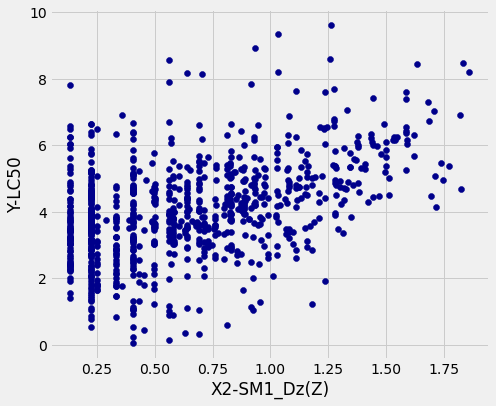
\includegraphics[width=\textwidth]{qsar_x2.png}
    	\caption{X2-SM1\_Dz(Z)}
    	\label{fig2:x2}
    	\end{subfigure}
    	\hfill
    	\begin{subfigure}[!htb]{0.25\textwidth}
		\centering
		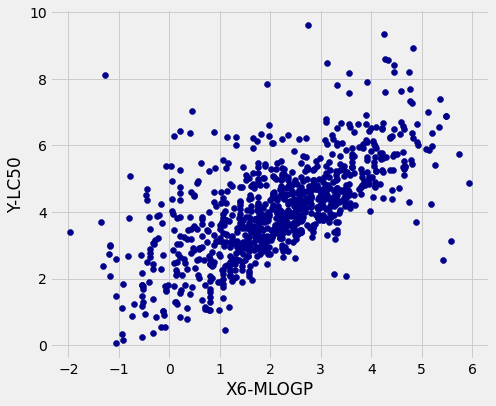
\includegraphics[width=\textwidth]{qsar_x6.png}
		\caption{X6-MLOGP}
		\label{fig2:x6}
		\end{subfigure}
    	\hfill
        \begin{subfigure}[!htb]{0.25\textwidth}
    	\centering
    	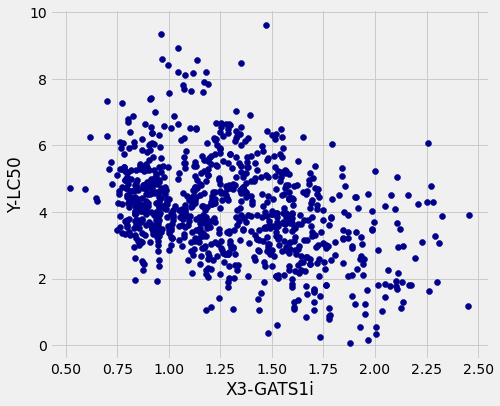
\includegraphics[width=\textwidth]{qsar_x3.png}
    	\caption{X3-GATS1i}
    	\label{fig2:x3}
    	\end{subfigure}
    	\label{fig2}	
    \end{figure}

	It is found that the linear association for every pair of independent and dependent variables from descending order are 0.6557147 (x6 and y), 0.44671574 (x2 and y), 0.29496689 (x1 and y), 0.1723897 (x4 and y), 0.17200377 (x5 and y), and -0.37377176 (x3 and y). This supports the initial inspection on the degree of correlation based on the scatter plots.

    \section{Regression algorithms}\label{sec:regression}
    
    This section covers simple and multiple regression with nearest neighbours and least squares. The idea of nearest neighbours is that if two points are near each other in the scatter-plot, then the corresponding measurements are most likely similar. Nearest neighbours is a model that assigns new data point based on the points within the neighbourhood that are most similar to it. The estimated y-value can be examined using the function: \emph{nn\_prediction(t, x\_col, y\_col, x\_val, x\_dist)}. The parameter t is the data table, \emph{x\_col} and \emph{y\_col} refers to the column of independent and dependent variable, \emph{x\_val} refers to the new data point, and \emph{x\_dist} refers to the threshold of distance. The return value is the average of the corresponding y-values for each group as the corresponding prediction.
    
    Least squares is a method to determine the best fit line to data, it involves using the slope-intercept formula: \emph{predicted\_y = (slope * x) + intercept}. The regression line aims to predict y-value given values of x however each line typically raises error in estimation. The line of "best" fit tries to obtain the smallest possible overall error among all straight lines. The prediction of y-value is determined applying the slope-intercept formula, using the optimum coefficients.
    
    Multiple regression is an extension to simple regression, it involves two or more independent variables. K-nearest neighbours is similar to nearest neighbours but the difference is that it returns top k training table at increasing order of the distances. The distance between two points is calculated using the Euclidean distance formula. The function for k nearest neighbours is: \emph{KNN\_model(y\_col, training, test, k)}. The parameter \emph{y\_col} is the column of the target variable, \emph{training} is the training data set which involves two or more independent variables, \emph{test} is the test data set, and \emph{k} is the chosen k-value. The returned value is the average of the observed y-values in these k training table.
    
    In the case of least squares, cost function is defined to quantify the error between predicted values and expected values. The cost function is specified as following: \emph{multiple\_regression\_rmse(var1\_coef, var2\_coef, var3\_coef, t, x1\_col, x2\_col, y\_col)}. The parameter \emph{var1\_coef} and \emph{var2\_coef} is the slope value for first and second explanatory variable, \emph{var3\_coef} is the intercept, \emph{t} is the training data, \emph{x1\_col} and \emph{x2\_col} is the column to the first and second explanatory variable, and \emph{y\_col} is the column to the target variable. The return value is the mean squared error (MSE) for the regression model. For simple and multiple regression, the minimize tool is used to search for the optimum coefficients. It tries to return the "best" coefficients by minimizing the mean squared error among all lines. 
    
    \section{Experiments and analysis}\label{sec:experiment}	
    	
	    \subsection{Simple Regression}\label{sec:simpleRegression}
	    The figure below displays scatter plots of original data points and prediction lines and residuals for nearest neighbours and least squares from a single independent variable: X6-MLOGP. 
	    
	    \begin{figure}[!htb]
		   	\centering
		    \begin{subfigure} [!htb]{0.3\textwidth}
		    	\centering
		    	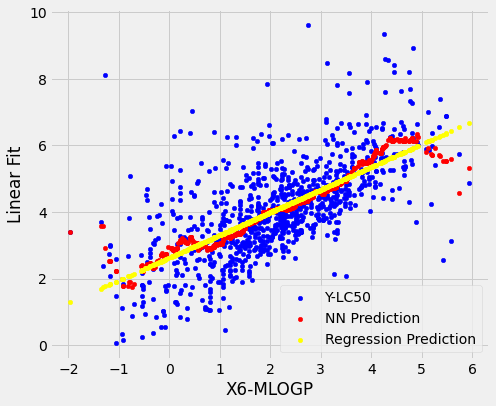
\includegraphics[width=0.8\textwidth]{simpleregression.png}	
		    	\caption{Nearest neighbours and least squares}
		    	\label{fig3:x1}	
		    \end{subfigure}
    		\qquad
		    \begin{subfigure} [!htb]{0.3\textwidth}
		    	\centering
		    	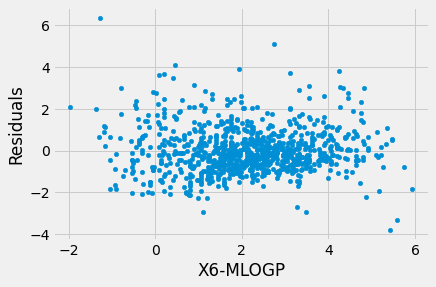
\includegraphics[width=0.8\textwidth]{simpleresiduals.png}	
		    	\caption{Residuals}
		    	\label{fig3:x2}
		    \end{subfigure}
		    \label{fig3}
		\end{figure}
		\newpage
		The residual plot shows no pattern or flat. This means that the residuals and predictor variable are uncorrelated, hence linear regression is a good alternative to solve the problem. The quality of regression can also be measured by accessing the numerical properties of residuals. Firstly, the correlation between the predictor variable and the residuals should be zero. Here, this value is -1.4e-15($\approx0$). Secondly, the average of the residuals should be zero. The actual result of the average of the residuals is 2.91e-15($\approx0$). Thirdly, the SD of the residuals should be a fraction of the SD of the response variable. This is also supported by the evidence where both values are equal to 1.094.
	    
	    The figure below shows result for nearest neighbours prediction and least squares. Graph A-C shows nearest neighbours prediction at a few different threshold values, the result shows that the predicted y-value is smaller as the threshold of distance is lower. When comparing the performance of least squares against nearest neighbours, it can be seen that the estimation of y-values given by both least squares and nearest neighbours are nearly similar.
	    
		\begin{figure}[!htb]
			\centering
			\begin{subfigure}[!htb]{0.45\textwidth}
				\centering
				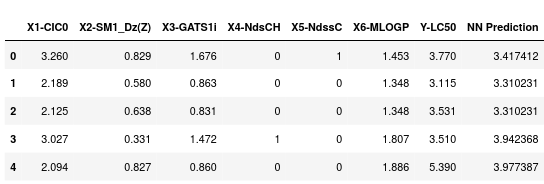
\includegraphics[width=\textwidth]{simple_nn_data1.png}
				\caption{Nearest neighbours at a threshold value of 0.2}
				\label{fig4:x1}
			\end{subfigure}
			\hfill
			\begin{subfigure}[!htb]{0.45\textwidth}
				\centering
				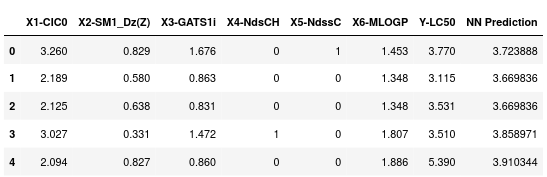
\includegraphics[width=\textwidth]{simple_nn_data2.png}
				\caption{Nearest neighbours at a threshold value of 1.5}
				\label{fig4:x2}
			\end{subfigure}
			\hfill
			\begin{subfigure}[!htb]{0.45\textwidth}
				\centering
				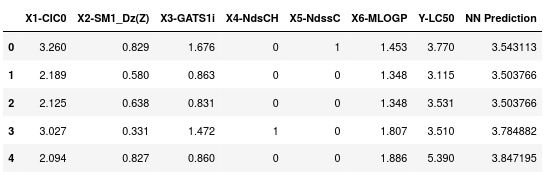
\includegraphics[width=\textwidth]{simple_nn_data3.png}
				\caption{Nearest neighbours at a threshold value of 0.75}
				\label{fig4:x3}
			\end{subfigure}
			\hfill
			\begin{subfigure}[!htb]{0.45\textwidth}
			\centering
			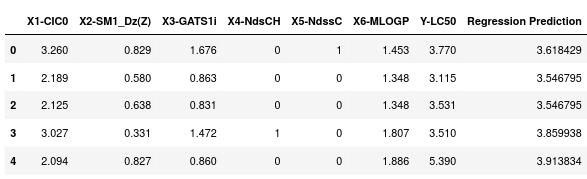
\includegraphics[width=\textwidth]{simple_ls_data.png}
			\caption{Least squares}
			\label{fig4:x4}
			\end{subfigure}
			\label{fig4}	
		\end{figure}

	    \subsection{Multiple Regression}\label{sec:multipleRegression}
	    
	    Table below shows the prediction accuracy of nearest neighbour at different value of k and least squares using different combinations of model inputs:
	    
	   	\begin{center}
		    \begin{tabular}{ |c|c|c|c|c|c| }
		    	\hline
		    	{Model Input} & \multicolumn{4}{|c|}{Nearest Neighbour} & {Least Squares} \\
		    	\hline
		    	{} & k=1 & k=3 & k=5 & k=11 & {} \\
		    	\hline
		    	x2 and x6 & 0.167 & 0.590 & 0.725 & 0.861 & 1.018 \\
		    	x1 and x6 & 0.162 & 0.671 & 0.854 & 1.012 & 1.093 \\
		    	x1 and x2 & 0.284 & 0.718 & 0.934 & 1.110 & 1.179 \\
		    	\hline
		    \end{tabular}
	    \end{center}
    
    	The result shows that the prediction accuracy for nearest neighbours is affected by tuning the parameter k and using different combinations of model inputs. It has been observed that for all model inputs, the mean squared error of estimation is greater when larger k-value is specified. For all cases, as a large k is specified, the errors for k-nearest neighbour is nearly similar to the least squares prediction. In contrast, k-nearest neighbour with a low k-value provides a lower value of errors, this indicates a better fit. Overall, the combination of variable x2 and x6 gives a lower MSE value compared to the other two model inputs, this suggests that the molecular component CIC0 and SM1\_Dz(Z) is a better measurement to predict the acute toxicity on fish. 
	    
	    \subsection{Bootstrapping}\label{sec:bootstrapping}
	    
	    With bootstrapping sample is drawn without replacement, each time the original data is resampled, a different predicted values for given value of x is returned. Bootstrapping estimates the properties of confidence intervals by measuring the data from a distribution. A confidence interval indicates that the prediction will likely to fall within a certain region. The figure below shows the histogram of 1000 bootstrap predictions for least squares in simple regression where x=2 using 96\% confidence level, the independent variable chosen here is X6-MLOGP. The empirical histogram is symmetric or bell-shaped, this means that the bootstrap percentile method works well for estimating confidence intervals. Furthermore, having a large sample size allows us to visualise a good probability distribution which result in decent approximations. By taking 96\% confidence level, the prediction interval ranges from 2th percentile to the 98th percentile of the predictions. The interval ranges from about 3.918 to 4.071. Using the original data, the predicted y-value is 3.992 which is roughly the centre of the interval. This range is narrow which suggests that the uncertainty in the estimation of y is statistically small. This is because the x-value is close to the centre of the distribution (mean=2.11). In general, instances are closer to each other near the mean of x and as a result the confidence interval is narrow.
	    
	    \begin{figure}[!htb]
	    		\centering
	    		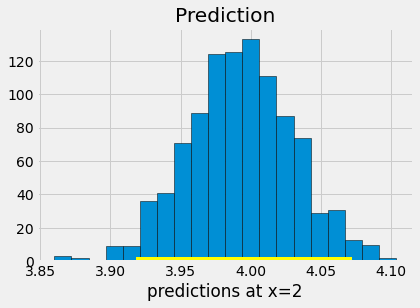
\includegraphics[width=0.3\textwidth]{hist_simple_1.png}	
	    		\label{fig5}
	    \end{figure}
    
	    The table below shows confidence interval obtained for predictions at a different value of x for simple regression of least squares using the same independent variable X6-MLOGP. It shows that the confidence interval are wider with x=-1 (0.478) and x=5 (0.396) compared to the x-values that are closer to the mean. It is assumed that instances are farther apart from each other at x=1 or x=5 compared to x=2 or x=3 and therefore the predictions varies as well.
    	\begin{center}
    	\begin{tabular}{||c c c c||} 
    		\hline
    		x=-1 & x=2 & x=3 & x=5 \\ [0.5ex] 
    		\hline\hline
    		0.478 & 0.154 & 0.173 & 0.396 \\ 
    		\hline
    	\end{tabular}
    	\end{center}
    
    	The figure below shows the histogram of 1000 bootstrap predictions for least squares in multiple regression at x1=3 and x2=1 where x1 represents X6-MLOGP, and x2 represents X2-SM1\_Dz(Z). The interval ranges from about 4.904 to 5.114, the predicted y-value based on the original table data is 5.001 which lies within the interval range. The confidence interval above using a single variable MLOGP is slightly narrower than combining MLOGP and SM1\_Dz(Z). This might suggests that using one explanatory variable is enough to measure the concentration that causes death in fish.
    	\begin{figure}[!htb]
    	\centering
    	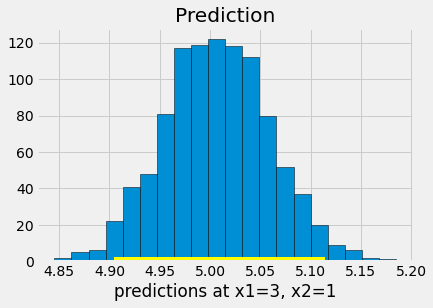
\includegraphics[width=0.3\textwidth]{hist_mult_1.png}	
    	\label{fig5}
    	\end{figure}
    \newpage
    \section{Conclusion}\label{sec:conclusion}
    
    This assignment aims to implement simple and multiple regression model with nearest neighbour and least squares approaches to evaluate acute toxicity on fish based on the data retrieved from UCI Machine Learning site. Several explanatory variables have been explored to predict acute toxicity on fish. Among all explanatory variables, it is found that there is a stronger relationship between MLOGP (molecular properties) with LC50, a concentration that causes death in fish. The properties of residuals in regression analysis show that linear regression is a suitable method to solve the problem. Experiments were carried out to find the prediction accuracies for nearest neighbour and least squares. It is concluded that there are many factors to predict Y-LC50 this can be in the approach measurement or the combination of model inputs.
 	
 	I am satisfied with the outcome of the report, however if I would have done it differently, I would allocate more time to prepare the evaluation report. There is a part which I missed and that is testing the prediction accuracies for simple regression. This is because I did not pay close attention to the question. 
    
    % Setting up your bibliography style - NOTE CMP uses Harvard style so stick with apalike for now
    \bibliographystyle{apalike}
    % Link your bibliography to your main.tex
	\bibliography{myBib.bib}
	% Look at DBLP or Google Scholar for references (NOTE - Google Scholar can produce usable bib entries - allowing you to copy and paste into myBib.bib)
	

\end{document}

